% !TEX TS-program = xelatexmk

\documentclass[12pt]{myNotes}

%%%%%%%%%%%%%%%%%%%%%%%%%%%%%%%%%%%%%%%%%%%%%%%%%%%%%%%%%%%%%%%%%%%%%%%%%%%
\usepackage[english]{babel}
\hyphenation{TOPPView}
\hyphenation{KNIME}
\hyphenation{OpenMS}

%%%%%%%%%%%%%%%%%%%%%%%%%%%%%%%%%%%%%%%%%%%%%%%%%%%%%%%%%%%%%%%%%%%%%%%%%%%
% FONT SELECTION -> WE NOW USE UBUNTU FONT AND XETEX FOR A MORE PROFESSIONAL
% LOOK.
% UBUNTU FONT CAN BE DOWNLOADED FROM HERE: http://font.ubuntu.com
%
\usepackage{fontspec}
\setmainfont[Ligatures = TeX]{Ubuntu-R.ttf}
\setmonofont[Ligatures = TeX]{Ubuntu-M.ttf}

% math fonts
%\usepackage[math-style=TeX]{unicode-math}
%\setmathfont{Cambria Math}


%%%%%%%%%%%%%%%%%%%%%%%%%%%%%%%%%%%%%%%%%%%%%%%%%%%%%%%%%%%%%%%%%%%%%%%%%%%
\usepackage{amsmath,amssymb,amscd,bm,dsfont,wasysym}
\usepackage{graphicx}
\usepackage[xetex,
      colorlinks=false,
      urlcolor=black,       % \href{...}{...} external (URL)
      filecolor=black,     % \href{...} local file
      linkcolor=black,       % \ref{...} and \pageref{...}
      citecolor=black,
      pdftitle={OpenMS Tutorial Handouts},
      pdfauthor={Johannes Veit},
      pdfsubject={},
      pdfkeywords={},
      pagebackref,
      pdfpagemode=none,
      bookmarksopen=true]{hyperref}

%%%%%%%%%%%%%%%%%%%%%%%%%%%%%%%%%%%%%%%%%%%%%%%%%%%%%%%%%%%%%%%%%%%%%%%%%%%

\newfontfamily{\menlo}{Menlo-Regular.ttf}

\usepackage{listings}
\usepackage{color}
\usepackage{textcomp}
\definecolor{listinggray}{gray}{0.9}
\definecolor{lbcolor}{rgb}{0.9,0.9,0.9}
\lstset{
    backgroundcolor=\color{lbcolor},
    tabsize=4,
    rulecolor=,
    language=python,
    basicstyle=\menlo\scriptsize,
    upquote=true,
    aboveskip={1.5\baselineskip},
    columns=fixed,
    showstringspaces=false,
    extendedchars=true,
    breaklines=true,
    prebreak = \raisebox{0ex}[0ex][0ex]{\ensuremath{\hookleftarrow}},
    frame=single,
    showtabs=false,
    showspaces=false,
    showstringspaces=false,
    identifierstyle=\menlo,
    keywordstyle=\color[rgb]{0,0,1},
    commentstyle=\color[rgb]{0.133,0.545,0.133},
    stringstyle=\color[rgb]{0.627,0.126,0.941},
}

%%%%%%%%%%%%%%%%%%%%%%%%%%%%%%%%%%%%%%%%%%%%%%%%%%%%%%%%%%%%%%%%%%%%%%%%%%%
% only use those two in combination
\usepackage[textsize=scriptsize]{todonotes}
%\usepackage[firstpage]{draftwatermark}
%\SetWatermarkScale{4}

%%%%%%%%%%%%%%%%%%%%%%%%%%%%%%%%%%%%%%%%%%%%%%%%%%%%%%%%%%%%%%%%%%%%%%%%%%%
% better key and menu tips
\usepackage{menukeys}
\renewmenumacro{\directory}[/]{pathswithfolder}

%%%%%%%%%%%%%%%%%%%%%%%%%%%%%%%%%%%%%%%%%%%%%%%%%%%%%%%%%%%%%%%%%%%%%%%%%%%
% easy referencing
\usepackage[noabbrev,capitalise]{cleveref}

%%%%%%%%%%%%%%%%%%%%%%%%%%%%%%%%%%%%%%%%%%%%%%%%%%%%%%%%%%%%%%%%%%%%%%%%%%%
% subfigures
\usepackage{subcaption}

%%%%%%%%%%%%%%%%%%%%%%%%%%%%%%%%%%%%%%%%%%%%%%%%%%%%%%%%%%%%%%%%%%%%%%%%%%%
% boxes with notes
%%%%%%%%%%%%%%%%%%%%%%%%%%%%%%%%%%%%%%%%%%%%%%%%%%%%%%%%%%%%%%%%%%%%%%%%%%%
\usepackage{tikz}
\usetikzlibrary[shadows]
\usepackage[framemethod=TikZ]{mdframed}
\usetikzlibrary{calc}

\global\mdfdefinestyle{notedefault}{topline=false,bottomline=false,rightline=false,leftmargin=1cm}
\newcommand{\note}[1]{ \begin{mdframed}[style=notedefault] \textbf{Note:}~#1 \end{mdframed} }

%%%%%%%%%%%%%%%%%%%%%%%%%%%%%%%%%%%%%%%%%%%%%%%%%%%%%%%%%%%%%%%%%%%%%%%%%%%
\newmdenv[
  leftmargin=0pt,
  rightmargin=20pt,
  innertopmargin=30pt,
  innerbottommargin=10pt,
  innerleftmargin=45pt,
  middlelinewidth=0pt,
  linecolor=black,
  topline=false,
  bottomline=false,
  rightline=false,
  font=\normalfont\normalsize,
  frametitlefont=\normalfont\normalsize\bfseries,
  frametitleaboveskip=1em,
  singleextra={
    \node[inner sep=0pt,anchor=north west,xshift=10pt,yshift=-30pt] at (P-|O) {\includegraphics[width=1.3cm]{graphics/assets/question23}};
    \node[inner sep=0pt,anchor=north west,yshift=-.8\baselineskip,font=\bfseries,xshift=10pt] at (P-|O) {Question};
  },
  firstextra={
    \node[inner sep=0pt,anchor=north west,xshift=10pt,yshift=-30pt] at (P-|O) {\includegraphics[width=1.3cm]{graphics/assets/question23}};
    \node[inner sep=0pt,anchor=north west,yshift=-.8\baselineskip,font=\bfseries,xshift=10pt] at (P-|O) {Question};
  }
]{question}

%%%%%%%%%%%%%%%%%%%%%%%%%%%%%%%%%%%%%%%%%%%%%%%%%%%%%%%%%%%%%%%%%%%%%%%%%%%
\newmdenv[
  leftmargin=0pt,
  rightmargin=20pt,
  innertopmargin=30pt,
  innerbottommargin=10pt,
  innerleftmargin=45pt,
  middlelinewidth=0pt,
  linecolor=black,
  topline=false,
  bottomline=false,
  rightline=false,
  font=\normalfont\normalsize,
  frametitlefont=\normalfont\normalsize\bfseries,
  frametitleaboveskip=1em,
  singleextra={
    \node[inner sep=0pt,anchor=north west,xshift=10pt,yshift=-30pt] at (P-|O) {\includegraphics[width=1.3cm]{graphics/assets/check30}};
    \node[inner sep=0pt,anchor=north west,yshift=-.8\baselineskip,font=\bfseries,xshift=10pt] at (P-|O) {Task};
  },
  firstextra={
    \node[inner sep=0pt,anchor=north west,xshift=10pt,yshift=-30pt] at (P-|O) {\includegraphics[width=1.3cm]{graphics/assets/check30}};
    \node[inner sep=0pt,anchor=north west,yshift=-.8\baselineskip,font=\bfseries,xshift=10pt] at (P-|O) {Task};
  }
]{task}

%%%%%%%%%%%%%%%%%%%%%%%%%%%%%%%%%%%%%%%%%%%%%%%%%%%%%%%%%%%%%%%%%%%%%%%%%%%
\newcommand{\KNIMENODE}[1]{\texttt{#1}}
\newcommand{\OPENMSTOOL}[1]{\texttt{#1}}

\begin{document}
%%%%%%%%%%%%%%%%%%%%%%%%%%%%%%%%%%%%%%%%%%%%%%%%%%%%%%%%%%%%%%%%%%%%%%%%%%%

\firstpages

%%%%%%%%%%%%%%%%%%%%%%%%%%%%%%%%%%%%%%%%%%%%%%%%%%%%%%%%%%%%%%%%%%%%%%%%%%%

\setcounter{equation}{0}
\section{General remarks}
\label{General remarks}

\begin{itemize}
\item This handout will guide you through an introductory tutorial for the OpenMS/TOPP software package~\cite{OpenMS}.
\item OpenMS~\cite{Sturm2008} is a versatile open-source library for mass spectrometry data analysis. Based on this library, we offer a collection
      of command-line tools ready to be used by end users. These so-called TOPP tools (short for ``The OpenMS Proteomics Pipeline'')~\cite{Kohlbacher2007} can be understood as
      small building blocks of arbitrary complex data analysis workflows.
\item In order to facilitate workflow construction, OpenMS was integrated into KNIME~\cite{KNIME}, the Konstanz
			Information Miner, an open-source integration platform providing a powerful and flexible workflow system
			combined with advanced data analytics, visualization, and report capabilities. Raw MS data as well as the
			results of data processing using TOPP can be visualized using TOPPView~\cite{Sturm2009}.
\item In this hands-on tutorial session, you will become familiar with some of the basic functionalities of OpenMS/TOPP, TOPPView, and KNIME
      and learn how to use a selection of TOPP tools used in the tutorial workflows.
\item All data referenced in this tutorial can be found in the \directory{Example\_Data} folder that came with this tutorial.
\end{itemize}

%%%%%%%%%%%%%%%%%%%%%%%%%%%%%%%%%%%%%%%%%%%%%%%%%%%%%%%%%%%%%%%%%%%%%%%%%%%
%\newpage
%!TEX root = handout.tex

\setcounter{equation}{0}

%%%%%%%%%%%%%%%%%%%%%%%%%%%%%%%%%%%%%%%%%%%%%%%%%%%%%%%%%%%%%%%%%%%%%%%%%%%%%%%%
\section{Getting started}

\subsection{Data conversion}
\label{Data_Conversion}

Each MS instrument vendor has one or more formats for storing the acquired data. Converting these data into an open format (preferably mzML) is the very first step when you want to work with open-source mass spectrometry software. A freely available conversion tool is ProteoWizard. The OpenMS installation package for Windows automatically installs ProteoWizard, so you do not need to download and install it separately.

Please note that due to restrictions from the instrument vendors, file format conversion for most formats is only possible on Windows systems, so exporting from the acquisition PC connected to the instrument is usually the most convenient option.
All files used in this tutorial have already been converted to mzML by us, so you do not need to do it yourself.

%%%%%%%%%%%%%%%%%%%%%%%%%%%%%%%%%%%%%%%%%%%%%%%%%%%%%%%%%%%%%%%%%%%%%%%%%%%%%%%%

\subsection{Data visualization using \OPENMSTOOL{TOPPView}}
\label{Data_Visualization}

Visualizing the data is the first step in quality control, an essential tool in understanding the data, and of course an essential step in pipeline development.
OpenMS provides a convenient viewer for some of the data: \OPENMSTOOL{TOPPView}.

We will guide you through some of the basic features of \OPENMSTOOL{TOPPView}. Please familiarize yourself with the key controls and visualization methods.
We will make use of these later throughout the tutorial. Let's start with a first look at one of the files of our tutorial data set:

\begin{itemize}
\item Start \OPENMSTOOL{TOPPView} (see Start-Menu or Applications on MacOS)
\item Go to \menu{File > Open File}, navigate to the directory where you copied the contents of the USB stick to,
      and select
      \directory{ OpenMS / small / velos005614.mzML}
      . This file contains a reduced LC-MS map (only a selected RT and m/z range
      was extracted using the TOPP tool FileFilter) of a label-free measurement of the human platelet proteome recorded on an Orbitrap velos.
      The other two mzML files contain technical replicates of this experiment.
\item Play around.
\item Three action modes are supported, one for scrolling, one for zooming and one for measuring:
    \begin{itemize}
    \item Scroll mode
        \begin{itemize}
        \item It is activated by default, though each loaded spectra file is displayed zoomed out first, so you do not need to scroll.
        \item When zommed in, to scroll the spectra map, click-drag on the current view.
        \item Arrow keys can be used to scroll the view as well.
        \end{itemize}
    \item Zoom mode
        \begin{itemize}
        \item All previous zoom levels are stored in a zoom history. The zoom history can be traversed using
              \keys[,]{\ctrl,+} or \keys[,]{\ctrl,-} or the mouse wheel (scroll up and down).
        \item Zooming into the data: either mark an area in the current view with your mouse while holding the left mouse
              button plus the \keys{\ctrl} key to zoom to this area
              or use your mouse wheel to traverse the zoom history.
        \item If you have reached the end of the history and keep on pressing \keys[,]{\ctrl,+} or
        			scroll up, the current area will be enlarged by a factor of $1.25$
        \item Pressing the Backspace key resets the zoom and zoom history.
        \end{itemize}
    \item Measure mode
        \begin{itemize}
        \item It is activated using the \keys{\shift} key.
        \item Press the left mouse button down while a peak is selected and drag the mouse to
        			another peak to measure the distance between peaks.
        \item This mode is implemented in the 1D and 2D mode only.
        \end{itemize}
    \end{itemize}
\item Right click on your 2D map and select \menu{Switch to 3D view} and examine your
			data in 3D mode
\item Go back to the 2D view. In 2D mode, visualize your data in different normalization modes, use linear, percentage and log-view (icons on the upper left tool bar).
\note{On \textit{Apple OS X}, due to a bug in one of the external libraries used by OpenMS, you will see a small window of the 3D mode when switching to 2D. Close the 3D tab in order to get rid of it.}
\item In \OPENMSTOOL{TOPPView} you can also execute TOPP tools. Go to
			\menu{Tools > Apply tool (whole layer)} and choose a TOPP tool (e.g., FileInfo) and
			inspect the results.
\end{itemize}

%%%%%%%%%%%%%%%%%%%%%%%%%%%%%%%%%%%%%%%%%%%%%%%%%%%%%%%%%%%%%%%%%%%%%%%%%%%%%%%%

\subsection{Introduction to KNIME / OpenMS}
\label{KNIME_Intro}

Using OpenMS in combination with KNIME you can create, edit, open, save, and run workflows
combining TOPP tools with the powerful data analysis capabilities of KNIME. Workflows can
be created conveniently in a graphical user interface. The parameters of all involved
tools can be edited within the application and are also saved as part of the workflow.
Furthermore, KNIME interactively performs validity checks during the workflow editing
process, in order to make it more difficult to create an invalid workflow.

Throughout most of the parts of this tutorial you will use KNIME to create and
execute workflows. This first step is to make yourself familiar with KNIME.

\subsubsection{Install OpenMS using KNIME}

Before we can start with the tutorial we need to install all the required extension for KNIME.
First we will install the OpenMS plugin, providing all the OpenMS nodes.
Afterwards we will install some additional plugins that we will use in the more advanced part of this tutorial.

\begin{enumerate}
\item Open KNIME.
\item Click on \menu{Help > Install New Software...}
\item \label{it:add_site} In the now open dialog choose \menu{Add...} (in the upper right corner of the dialog) to define a new update site. In the opening dialog enter the following details. \\
\textit{Name:} \texttt{Trunk Community Contributions} \\
\textit{Location:} \texttt{http://tech.knime.org/update/community-contributions/trunk/}
\item \label{it:select_site} After pressing \keys{OK} KNIME will show you all the contents of the added Update Site, containing also the OpenMS nodes.
%\todo{First install File Handling Nodes?}
\item Select the OpenMS nodes in the category "KNIME Community Contributions - Bioinformatics \& NGS" and click \keys{Next}.
\item Follow the instructions and after a restart of KNIME the OpenMS nodes will be available under “Community Nodes”.
\end{enumerate}

\note{
For this tutorial we use a pre-release version of OpenMS 1.12.
While not being a full release, it was nevertheless intensively tested to ensure its functionality for this tutorial.
For regular use we recommend using the latest stable OpenMS release.
To install the latest stable release skip Steps \ref{it:add_site} and \ref{it:select_site} and instead choose the update site \menu{Trusted Community Contributions}.
Please note that some of the workflows shown here require OpenMS 1.12 and therefore will not work with OpenMS 1.11.1 downloaded from the stable update site.
}

For the rest of the tutorial we will also need some more plugins, that can be installed similar to the OpenMS nodes.

\begin{enumerate}
\item Again, click on \menu{Help > Install New Software...}
\item From the \menu{Work with:} drop down list select the \menu{KNIME Analytics Platform Update Site}
\item Now select the following plugins from the \textit{KNIME \& Extensions} category
    \begin{itemize}
    \item KNIME Base Chemistry Types \& Nodes
    \item KNIME Chemistry Add-Ons
    \item KNIME File Handling Nodes
    \item KNIME Interactive R Statistics Integration
    \item KNIME Math Expression (JEP)
    \item KNIME Report Designer
    \item KNIME SVG Support
    \item KNIME XLS Support
    \item KNIME XML-Processing
    \end{itemize}
\item And the following plugin from the \textit{Marvin Chemistry Extensions (donated by Infocom \& Chemaxon)} category
    \begin{itemize}
    \item ChemAxon/Infocom Marvin Extensions Feature
    \end{itemize}
\item Click \keys{Next} and follow the instructions.
\end{enumerate}

\subsubsection{KNIME Concepts}

A \textbf{workflow} is a sequence of steps applied to a single or multiple input data sets to process and analyse this data.
In KNIME such workflows are implemented graphically by combining so-called \textbf{nodes}.

A node represents a single analysis step in a workflow.
Nodes have input and output ports where the data goes into to the node or the results are provided for other nodes after processing, respectively.
KNIME distinguishes between different port types, representing different types of data.
The most common representation in KNIME are tables (similar to an excel sheet).
Those ports are marked with a small triangle.
For OpenMS we use a different port type, so called file ports, representing complete files.
Those ports are marked by a small grey box.
Dark grey boxes represent mandatory inputs and light grey boxes optional inputs.

Nodes can have three different states, indicated by the small traffic light below the node.

\begin{itemize}
\item
Inactive, failed, and not yet fully configured nodes are marked red.
\item
Configured but not yet executed nodes are marked yellow.
\item
Successfully executed nodes are marked green.
\end{itemize}

If the node execution failed the node will switch to the red state.

Most nodes will be configured as soon as all input ports are connected.
For some nodes additional parameters have to be provided that cannot be either guessed from the data or filled with sensible defaults.
In this case, of if you want to customise the default configuration, you can open the configuration dialog of a node with a double-click on the node.
For OpenMS you will see a configuration dialog like the one shown in \cref{fig:knime_configure}.
\note{OpenMS distinguishes between normal parameters and advanced parameters.
Advanced parameters are by default hidden from the users since they should only rarely be customised.
In case you want to have a look at the parameters or need to customise them in one of the tutorials you can show them by clicking on the checkbox  \menu{Show advanced parameter} in the lower part of the dialog.}
The dialog shows the individual parameters, their current value and type, and, in the lower part of the dialog, the documentation for the currently selected parameter.

\begin{figure}
\centering
\includegraphics[width=0.5\textwidth]{graphics/knime_setup/knime_configure_dialog}
\caption{Node configuration dialog of an OpenMS node.}
\label{fig:knime_configure}
\end{figure}

\subsubsection{Overview of the graphical user interface}

\begin{figure}
\includegraphics[width=\textwidth]{graphics/knime_setup/knime_workbench_marked}
\caption{The KNIME workbench.}
\label{fig:knime_workbench}
\end{figure}

The graphical user interface (GUI) of KNIME consists of different components or so called panels that are shown in \cref{fig:knime_workbench}.
We will shortly introduce the individual panels and their purpose below.

\begin{description}
\item[Workflow Editor]
The workflow editor is the central part of the KNIME GUI.
Here you assemble the workflow by adding nodes from the Node Repository via "drag \& drop".
Nodes can be connected by clicking on the output port of one node and releasing the mouse at the desired input port of the next node.

\item[Workflow Explorer]
Shows a list of available workflows (also called workflow projects).
You can open a workflow by double clicking it.
A new workflow can be created with a right-click in the Workflow Explorer followed by selecting \menu{New KNIME Workflow...}.

\item[Node Repository]
Shows all nodes that are available in your KNIME installation.
Every plugin you install will provide new nodes that can be found here.
The OpenMS nodes can be found in \menu{Community Nodes > OpenMS}.
Nodes for managing files (e.g., Input Files or Output Folders) can be found in \menu{Community Nodes > GenericKnimeNodes}.
You can search the node repository by typing the node name into the small text box in the upper part of the node repository.

\item[Outline]
The Outline panel contains a small overview of the complete workflow. While of limited use when working on a small workflow, this feature is very helpful as soon as the workflows get bigger.

\item[Console]
In the console panel warning and error messages are shown.
This panel will provide helpful information if one of the nodes failed or shows an warnings sign.

\item[Node Description]
As soon as a node is selected, the Node Description window will show the documentation of the node including documentation for all its parameters.
For OpenMS nodes you will also find a link to the tool page in the online documentation.

\end{description}

\subsubsection{Creating workflows}
\label{sec:create_workflows}

Workflows can easily be created by a right click in the Workflow Explorer followed by clicking on \menu{New KNIME Workflow...}.

\subsubsection{Sharing workflows}
\label{sec:sharing_workflows}

To be able to share a workflow with others KNIME supports the import and export of complete workflows.
To export a workflow select it in the Workflow Explorer and select \menu{File > Export KNIME Workflow...}.
KNIME will export workflows as a zip file containing all the information on nodes, their connections, and their configuration.
Those zip files can again be imported by selecting \menu{File > Import KNIME Workflow...}.

\note{For your convenience we added all workflows discussed in this tutorial to the \directory{Workflows} folder.
If you want to check your own workflow by comparing it to the solution or got stuck, simply import the full workflow from the corresponding zip file.}

\subsubsection{Duplicating workflows}
\label{sec:duplicate-wf}

During the tutorial a lot of the workflows will be created based on the workflow from a previous task.
To keep the intermediate workflows we suggest you create copies of your workflows so you can see the progress.
To create a copy of your workflow follow the following steps

\begin{itemize}
\item
Right click on the workflow you want to create a copy of in the Workflow Explorer and select \menu{Copy}.
\item
Right click again somewhere on the workflow explorer and select \menu{Paste}.
\item
This will create a workflow with same name as the one you copied with a (2) appended.
\item
To distinguish them later on you can easily rename the workflows in the Workflow Explorer by right clicking on the workflow and selecting \menu{Rename}. \note{To rename a workflow it has to be closed.}
\end{itemize}

\subsubsection{A minimal workflow}
\label{Minimal_Workflow}

Let us now start with the creation of our very first, very simple workflow.
As a first step, we will gather some basic information about the data set before starting the
actual development of a data analysis workflow.

\begin{itemize}
\item
Create a new workflow.
\item Add an \KNIMENODE{Input File} node and an \KNIMENODE{Output Folder} node (to be found in \menu{Community Nodes > GenericKnimeNodes > IO} and a \KNIMENODE{FileInfo} node (to be found in the category \menu{Community Nodes > OpenMS > File Handling}) to the workflow.
\item Connect the \KNIMENODE{Input File} node to the \KNIMENODE{FileInfo} node, and the first output port of the \KNIMENODE{FileInfo} node to the \KNIMENODE{Output Folder} node.
\note{In case you are unsure about which node port to use, hovering the cursor over the port in question will display the port name and what kind of input it expects.}
The complete workflow is shown in \cref{fig:knime_minimal}.
FileInfo can produce two different kinds of output files.
\item All nodes are still marked red, since we are missing an actual input file.
Double-click the Input File node and select \menu{Browse}.
In the file system browser select \directory{OpenMS / tiny / velos005614.mzML} and click \menu{Open}.
Afterwards close the dialog by clicking \menu{Ok}.
\note{Make sure to use the ``tiny'' version this time, not ``small'', for the sake of faster workflow execution.}
\item The \KNIMENODE{Input File} node and the \KNIMENODE{FileInfo} node should now have switched to yellow, but the \KNIMENODE{Output Folder} node is still red.
Double-click on the \KNIMENODE{Output Folder} node and click on \menu{Browse} to select an output directory for the generated data.
\item Great! Your first workflow is now ready to be run. Press \keys{\shift + F7} to execute the complete workflow.
You can also right click on any node of your workflow and select \menu{Execute} from the context menu.
\item The traffic lights tell you about the current status of all nodes in your workflow.
Currently running tools show either a progress in percent or a moving blue bar, nodes waiting for data show the small word ``queued'', and successfully executed ones become green.
If something goes wrong (e.g., a tool crashes), the light will become red.
\item In order to inspect the results, you can just right-click the \KNIMENODE{Output Folder} node and select \menu{View: Open the output folder}.
You can then open the text file and inspect its contents.
You will find some basic information of the data contained in the mzML file, e.g., the total number of spectra and peaks, the RT and m/z range, and how many MS1 and MS2 spectra the file contains.
\end{itemize}

\begin{figure}
\centering
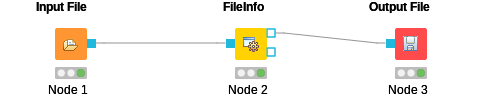
\includegraphics[width=0.59\textwidth]{graphics/knime_setup/Minimal_FileInfo}
\caption{A minimal workflow calling FileInfo on a single file.}
\label{fig:knime_minimal}
\end{figure}

Now consider you would like to gather this information for more then one file.
We will now modify the workflow to compute the same information on three different files and then write the output files to a folder.

\begin{itemize}
\item
We start from the previous workflow.
\item
First we need to replace our single input file with multiple files.
Therefore we add the \KNIMENODE{Input Files} node from the category \menu{Community Nodes > GenericKnimeNodes > IO}.
\item
To select the files we double-click on the \KNIMENODE{Input Files} node and click on \menu{Add}.
In the filesystem browser we select all three files from the directory \directory{OpenMS / tiny / }.
And close the dialog with \menu{Ok}.
\item
We now add two more nodes: the \KNIMENODE{ZipLoopStart} and the \KNIMENODE{ZipLoopEnd} node from the category \menu{Community Nodes > GenericKnimeNodes > Flow}.
\item
Afterwards we connect the \KNIMENODE{Input Files} node to the first port of the \KNIMENODE{ZipLoopStart} node, the first port of the \KNIMENODE{ZipLoopStart} node to the \KNIMENODE{FileInfo} node, the first output port of the \KNIMENODE{FileInfo} node to the first input port of the \KNIMENODE{ZipLoopEnd} node, and the first output port of the \KNIMENODE{ZipLoopEnd} node to the \KNIMENODE{Output Folder} node (, not \KNIMENODE{Output File}).
The complete workflow is shown in \cref{fig:knime_minimal_loop}
\item
The workflow is already complete.
Simply execute the workflow and inspect the output as before.
\end{itemize}

\begin{figure}
\centering
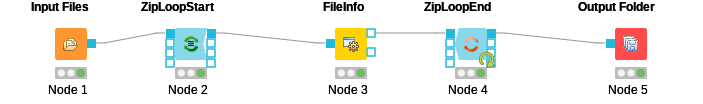
\includegraphics[width=\textwidth]{graphics/knime_setup/Minimal_FileInfoLoop}
\caption{A minimal workflow calling FileInfo on multiple files in a loop.}
\label{fig:knime_minimal_loop}
\end{figure}



%!TEX root = handout.tex

\newpage
\section{Label-free quantification of peptides}
\label{sec:lfq}

\subsection{Introduction}

In this chapter, we will build a workflow with OpenMS / KNIME to quantify a label-free experiment. 
Label-free quantification is a method aiming to compare the relative amounts of proteins or peptides in two or more samples.
We will start from the minimal workflow of the last chapter and, step-by-step, build a label-free quantification workflow.

\subsection{Peptide Identification}
\label{Peptide_Identification}

As a start, we will extend the minimal workflow so that it performs a peptide identification using the OMSSA~\cite{Geer:2004p285} search engine. Since OpenMS version 1.10, OMSSA is included in the OpenMS installation, so you do not need to download and install it yourself.

\begin{itemize}
\item Let's start by replacing the input files in our \KNIMENODE{Input Files} node by the three mzML files in \directory{Example\_Data / Labelfree / datasets / lfq\_spikein\_dilution\_1-3.mzML}. This is a reduced toy dataset where each of the three runs contains a constant background of \textit{S. pyogenes} peptides as well as human spike-in peptides in different concentrations.~\cite{Chawade:2015}
\item Instead of FileInfo, we want to perform OMSSA identification, so we simply replace the \KNIMENODE{FileInfo} node with the \KNIMENODE{OMSSAAdapter} node \menu{Community Nodes > OpenMS > Identification}, and we are almost done. Just make sure you have connected the \KNIMENODE{ZipLoopStart} node with the \texttt{in} port of the \KNIMENODE{OMSSAAdapter} node.
\item OMSSA, like most mass spectrometry identification engines, relies on searching the input spectra against sequence databases. Thus, we need to introduce a search database input. As we want to use the same search database for all of our input files, we can just add a single \KNIMENODE{Input File} node to the workflow and connect it directly with the \KNIMENODE{OMSSAAdapter} \texttt{database} port. KNIME will automatically reuse this Input node each time a new ZipLoop iteration is started. In order to specify the database, select \directory{Example\_Data / Labelfree / databases / \\ s\_pyo\_sf370\_potato\_human\_target\_decoy\_with\_contaminants.fasta}, and we have a very basic peptide identification workflow.
%\note{We recommend to choose a different output directory every time you extend and run your pipeline again.}
\note{You might also want to save your new identification workflow under a different name. Have a look at \cref{sec:duplicate-wf} for information on how to create copies of workflows.}
\item The result of a single OMSSA run is basically a number of peptide-spectrum-matches (PSM) with a score each, and these will be stored in an idXML file. Now we can run the pipeline and after execution is finished, we can have a first look at the results: just open the input files folder with a file browser and from there open an mzML file in \OPENMSTOOL{TOPPView}.
\item Here, you can annotate this spectrum data file with the peptide identification results. Choose \menu{Tools > Annotate with identification} from the menu and select the idXML file that \KNIMENODE{OMSSAAdapter} generated (it is located within the output directory that you specified when starting the pipeline).
\item On the right, select the tab \menu{Identification view}. Using this view, you can see all identified peptides and browse the corresponding MS2 spectra.
\note{Opening the output file of \KNIMENODE{OMSSAAdapter} (the idXML file) directly is also possible, but the direct visualization of an idXML file is less useful.}
\item The search results stored in the idXML file can also be read back into a KNIME table for inspection and subsequent analyses: Add a \KNIMENODE{TextExporter} node from \menu{Community Nodes > OpenMS > File Handling} to your workflow and connect the output port of your \KNIMENODE{OMSSAAdapter} (the same port your \KNIMENODE{ZipLoopEnd} is connected to) to its input port. This tool will convert the idXML file to a more human-readable text file which can also be read into a KNIME table using the \KNIMENODE{IDTextReader} node. Add an \KNIMENODE{IDTextReader} node (\menu{Community Nodes > OpenMS > Conversion}) after \KNIMENODE{TextExporter} and execute it. Now you can right-click \KNIMENODE{IDTextReader} and select \menu{ID Table} to browse your peptide identifications.
\item From here, you can use all the tools KNIME offers for analyzing the data in this table. As a simple example, you could add a \KNIMENODE{Histogram} node (from category \menu{Data Views}) node after \KNIMENODE{IDTextReader}, double-click it, select \textit{peptide\_charge} as binning column, hit \menu{OK}, and execute it. Right-clicking and selecting \menu{View: Histogram view} will open a plot showing the charge state distribution of your identifications.
\end{itemize}

In the next step, we will tweak the parameters of OMSSA to better reflect the instrument's accuracy. Also, we will extend our pipeline with a false discovery rate (FDR) filter to retain only those identifications that will yield an FDR of $<$ 1 \%.

\begin{itemize}
\item
Open the configuration dialog of \KNIMENODE{OMSSAAdapter}.
The dataset was recorded using an LTQ Orbitrap XL mass spectrometer, so we can set the precursor mass tolerance to a smaller value, say 10 ppm.
Set \textit{precursor\textunderscore mass\textunderscore tolerance} to 10 and \\ \textit{precursor\textunderscore error\textunderscore units} to \textit{ppm}.
\note{Whenever you change the configuration of a node, the node as well as all its successors will be reset to the Configured state (all node results are discarded and need to be recalculated by executing the nodes again).}
\item
Set \textit{max\_precursor\_charge} to 5, in order to also search for peptides with charges up to 5.
\item
Add \textit{Carbamidomethyl (C)} as fixed modification and \textit{Oxidation (M)} as variable modification.
\note{To add a modification click on the empty value field in the configuration dialog to open the list editor dialog.
In the new dialog click \menu{Add}.
Then select the newly added modification to open the drop down list where you can select the correct modification.}
\item
A common step in analyis is to search not only against a regular protein database, but to also search against a decoy database for FDR estimation.
The fasta file we used before already contains such a decoy database.
For OpenMS to know which OMSSA PSM came from which part of the file (i.e. target versus decoy), we have to index the results.
Therefore, extend the workflow with a \KNIMENODE{PeptideIndexer} node \menu{Community Nodes > OpenMS > ID Processing}.
This node needs the idXML as input as well as the database file.
\note{You can direct the files of an \KNIMENODE{Input File} node to more than just one destination port.}
\item
The decoys in the database are prefixed with ``DECOY\_'', so we have to set \textit{decoy\_string} to \textit{DECOY\_} and \textit{decoy\_string\_position} to \textit{prefix} in the configuration dialog of \KNIMENODE{PeptideIndexer}.
\item
Now we can go for the FDR estimation, which the \KNIMENODE{FalseDiscoveryRate} node will calculate for us (you will find it in \menu{Community Nodes > OpenMS > ID Processing}).
As we have a combined search database and thus only one idXML per mzML we will only use the \textit{in} port of the \KNIMENODE{FalseDiscoveryRate} node.
\item
In order to set the FDR level to $1\%$, we need an \KNIMENODE{IDFilter} node from \menu{Community Nodes > OpenMS > ID Processing}.
Configuring its parameter \textit{score $\rightarrow$ pep} to $0.01$ will do the trick.
The FDR calculations (embedded in the idXML) from the \KNIMENODE{FalseDiscoveryRate} node will go into the \textit{in} port of the \KNIMENODE{IDFilter} node.
\item
Execute your workflow and inspect the results using \KNIMENODE{IDTextReader} like you did before.
How many peptides did you identify at this FDR threshold?
\note{The finished identification workflow is now sufficiently complex that we might want to encapsulate it in a Meta node.
For this, select all nodes inside the ZipLoop (including the \KNIMENODE{Input File} node) and right-click to select \menu{Collapse into Meta node} and name it ID.
Meta nodes are useful when you construct even larger workflows and want to keep an overview.}
\end{itemize}

\begin{figure}[htbp]
  \centering
  \includegraphics[width=\textwidth]{graphics/labelfree/PepIdFDR.png}
  \caption{OMSSA ID pipeline including FDR filtering.}
  \label{fig:id_fdr}
\end{figure}

\subsubsection{Bonus task: identification using several search engines}
\note{If you are ahead of the tutorial or later on, you can further improve your FDR identification workflow by a so-called consensus identification using several search engines. Otherwise, just continue with section \ref{Labelfree_Quantification}.}
It has become widely accepted that the parallel usage of different search engines can increase peptide identification rates in shotgun proteomics experiments. The ConsensusID algorithm is based on the calculation of posterior error probabilities (PEP) and a combination of the normalized scores by considering missing peptide sequences.

\begin{itemize}
\item
Next to the \KNIMENODE{OMSSAAdapter} add a \KNIMENODE{XTandemAdapter} \\
\menu{Community Nodes > OpenMS > Identification} node and set its parameters and ports analogously to the \KNIMENODE{OMSSAAdapter}. In XTandem, to get more evenly distributed scores, we decrease the number of candidates a bit by setting the precursor mass tolerance to 5 ppm and the fragment mass tolerance to 0.1 Da.
\item
To calculate the PEP, introduce each a \KNIMENODE{IDPosteriorErrorProbability} \menu{Community Nodes > OpenMS > ID Processing} node to the output of each ID engine adapter node.
This will calculate the PEP to each hit and output an updated idXML.
\item
To create a consensus, we must first merge these two files with a \KNIMENODE{FileMerger} node \menu{Community Nodes > GenericKnimeNodes > Flow} so we can then merge the corresponding IDs with a \KNIMENODE{IDMerger} \menu{Community Nodes > OpenMS > File Handling}.
\item
Now we can create a consensus identification with the \KNIMENODE{ConsensusID} \menu{Community Nodes > OpenMS > ID Processing} node.
We can connect this to the \KNIMENODE{PeptideIndexer} and go along with our existing FDR filtering.
\note{By default, X!Tandem takes additional enzyme cutting rules into consideration (besides the specified tryptic digest). Thus for the tutorial files, you have to set PeptideIndexer's \textit{enzyme $\rightarrow$ specificity} parameter to \texttt{none} to accept X!Tandems non-tryptic identifications as well.}
\end{itemize}

\begin{figure}[htbp]
  \centering
  \includegraphics[width=\textwidth]{graphics/labelfree/PepConsensusId.png}
  \caption{Complete consensus identification workflow.}
  \label{fig:consensusid}
\end{figure}

\newpage
\subsection{Quantification}
\label{Labelfree_Quantification}

Now that we have successfully constructed a peptide identification pipeline, we can add quantification capabilities to our workflow.

\begin{itemize}
\item
Add a \KNIMENODE{FeatureFinderCentroided} node from \menu{Community Nodes > OpenMS > Quantitation} which gets input from the first output port of the \KNIMENODE{ZipLoopStart} node. Also, add an \KNIMENODE{IDMapper} node (from \menu{Community Nodes > OpenMS > ID Processing}) which receives input from the \KNIMENODE{FeatureFinderCentroided} node and the ID Meta node (or \KNIMENODE{IDFilter} node if you haven't used the Meta node).
The output of the \KNIMENODE{IDMapper} is then connected to an \textit{in} port of the \KNIMENODE{ZipLoopEnd} node.
\item
\KNIMENODE{FeatureFinderCentroided} finds and quantifies peptide ion signals contained in the MS1 data.
It reduces the entire signal, i.e., all peaks explained by one and the same peptide ion signal, to a single peak at the maximum of the chromatographic elution profile of the monoisotopic mass trace of this peptide ion and assigns an overall intensity.
\item
\KNIMENODE{FeatureFinderCentroided} produces a featureXML file as output, containing only quantitative information of so-far unidentified peptide signals.
In order to annotate these with the corresponding ID information, we need the \KNIMENODE{IDMapper} node.
\item Run your pipeline and inspect the results of the \KNIMENODE{IDMapper} node in TOPPView. Open the mzML file of your data to display the raw peak intensities.
\item To assess how well the feature finding worked, you can project the features contained in the featureXML file on the raw data contained in the mzML file. To this end, open the featureXML file in TOPPView by clicking on \menu{File > Open file} and add it to a new layer (\menu{Open in > New layer}). The features are now visualized on top of your raw data. If you zoom in on a small region, you should be able to see the individual boxes around features that have been detected (see Fig.~\ref{fig:ff_featurexml}). If you hover over the the feature centroid (small circle indicating the chromatographic apex of monoisotopic trace) additional information of the feature is displayed.

\begin{figure}[!htbp]
  \centering
  \includegraphics[width=0.85\textwidth]{graphics/labelfree/featureXML.png}
  \caption{Visualization of detected features (boxes) in TOPPView.}
  \label{fig:ff_featurexml}
\end{figure}

\note{The chromatographic RT range of a feature is about 30-60~s and its m/z range around 2.5 m/z in this dataset. If you have trouble zooming in on a feature, select the full RT range and zoom only into the m/z dimension by holding down \keys{\ctrlwin} (\keys{cmd \cmd} on macOS) and repeatedly dragging a narrow box from the very left to the very right.}
\item
You can see which features were annotated with a peptide identification by first selecting the featureXML file in the \texttt{Layers} window on the upper right side and then clicking on the icon with the letters A, B and C on the upper icon bar.
Now, click on the small triangle next to that icon and select \texttt{Peptide identification}.
\end{itemize}

\begin{figure}[htbp]
  \centering
  \includegraphics[width=\textwidth]{graphics/labelfree/PepQuantIdNoAlign.png}
  \caption{Extended workflow featuring peptide identification and quantification.}
  \label{fig:ff_idmapping}
\end{figure}

\subsection{Combining quantitative information across several label-free experiments}
\label{Combining}

So far, we successfully performed peptide identification as well as quantification on individual LC-MS runs. For differential label-free analyses, however, we need to identify and quantify corresponding signals in different experiments and link them together to compare their intensities. Thus, we will now run our pipeline on all three available input files and extend it a bit further, so that it is able to find and link features across several runs.

\begin{figure}[htbp]
  \centering
  \includegraphics[width=\textwidth]{graphics/labelfree/PepQuantId.png}
  \caption{Complete identification and label-free quantification workflow.}
  \label{fig:complete_without_consensusid}
\end{figure}

\begin{itemize}
    \item To find features across several maps, we first have to align them to correct for retention time shifts between the different label-free measurements. With the \KNIMENODE{MapAlignerPoseClustering} in \menu{Community Nodes > OpenMS > Map Alignment}, we can align corresponding peptide signals to each other as closely as possible by applying a transformation in the RT dimension. \note{\KNIMENODE{MapAlignerPoseClustering} consumes several featureXML files and its output should still be several featureXML files containing the same features, but with the transformed RT values. In its configuration dialog, make sure that \textit{OutputTypes} is set to featureXML.}
    \item With the \KNIMENODE{FeatureLinkerUnlabeledQT} node in \menu{Community Nodes > OpenMS > Map Alignment}, we can then perform the actual linking of corresponding features. Its output is a consensusXML file containing linked groups of corresponding features across the different experiments.
    \item Since the overall intensities can vary a lot between different measurements (for example, because the amount of injected analytes was different), we apply the \KNIMENODE{ConsensusMapNormalizer} in \menu{Community Nodes > OpenMS > Map Alignment} as a last processing step. Configure its parameters with setting \textit{algorithm\_type} to \texttt{median}. It will then normalize the maps in such a way that the median intensity of all input maps is equal.
    \item Finally, we export the resulting normalized consensusXML file to a csv format using \KNIMENODE{TextExporter}. Connect its out port to a new \KNIMENODE{Output Folder} node.
    \note{You can specify the desired column separation character in the parameter settings (by default, it is set to `` '' (a space)). The output file of \KNIMENODE{TextExporter} can also be opened with external tools, e.g., Microsoft Excel, for downstream statistical analyses.}
\end{itemize}

\subsubsection{Basic data analysis in KNIME}

For downstream analysis of the quantification results within the KNIME environment, you can use the \KNIMENODE{ConsensusTextReader} node in \menu{Community Nodes > OpenMS > Conversion} instead of the \KNIMENODE{Output Folder} node to convert the output into a KNIME table (indicated by a triangle as output port). 
After running the node you can view the KNIME table by right-clicking on the \KNIMENODE{ConsensusTextReader} and selecting \menu{Consensus Table}.
Every row in this table corresponds to a so-called consensus feature, i.e., a peptide signal quantified across several runs. The first couple of columns describe the consensus feature as a whole (average RT and m/z across the maps, charge, etc.). The remaining columns describe the exact positions and intensities of the quantified features separately for all input samples (e.g., intensity\_0 is the intensity of the feature in the first input file). The last 11 columns contain information on peptide identification.

\begin{figure}[htbp]
  \centering
  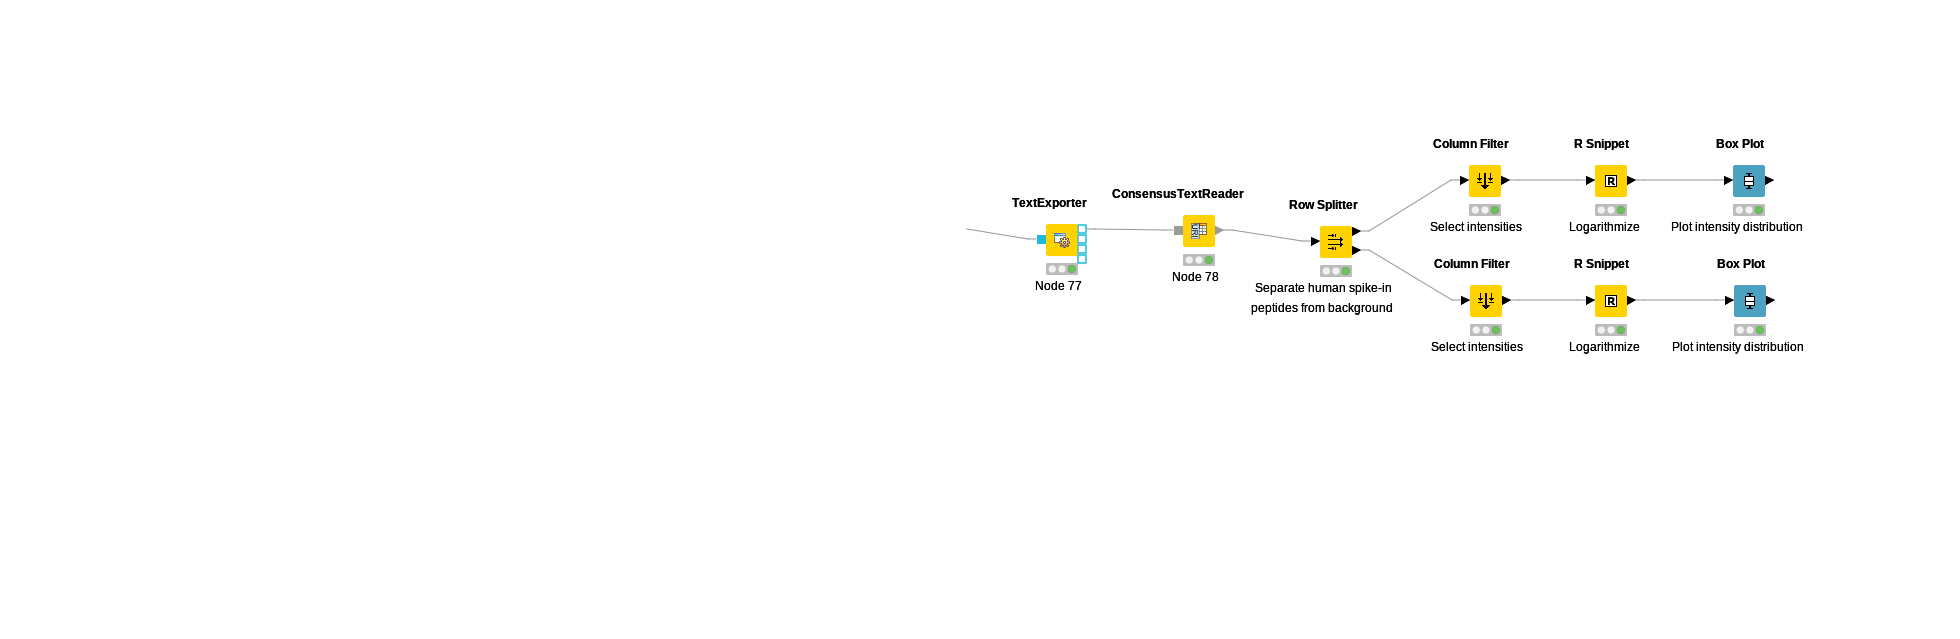
\includegraphics[width=0.85\textwidth]{graphics/labelfree/data_analysis.png}
  \caption{Simple KNIME data analysis example for LFQ.}
  \label{fig:lfq_data_analysis}
\end{figure}

\begin{itemize}
    \item Now, let's say we want to plot the log intensity distributions of the human spike-in peptides for all input files. In addition, we will plot the intensity distributions of the background peptides.
    \item As shown in Fig. \ref{fig:lfq_data_analysis}, add a \KNIMENODE{Row Splitter} node (\menu{Data Manipulation > Row > Filter}) after \KNIMENODE{ConsensusTextReader}. Double-click it to configure. The human spike-in peptides have accessions starting with ``hum''. Thus, set the column to apply the test to: \textit{accessions}, select pattern matching as matching criterion, enter \textit{hum*} into the corresponding text field, and check the \textit{contains wild cards} box. Press OK and execute the node.
    \item \KNIMENODE{Row Splitter} produces two output tables: the first one contains all rows from the input table matching the filter criterion, and the second table contains all other rows. You can inspect the tables by right-clicking and selecting \textit{Filtered} and \textit{Filtered Out}. The former table should now only contain peptides with a human accession, whereas the latter should contain all remaining peptides (including unidentified ones).
    \item Now, since we only want to plot intensities, we can add a \KNIMENODE{Column Filter} node \\ \menu{Data Manipulation > Column > Filter}, connect its input port to the \textit{Filtered} output port of the \KNIMENODE{Row Filter}, and open its configuration dialog. We could either manually select the columns we want to keep, or, more elegantly, select \textit{Wildcard/Regex Selection} and enter \textit{intensity\_?} as the pattern. KNIME will interactively show you which columns your pattern applies to while you're typing.
    \item Since we want to plot log intensities, we will now compute the log of all intensity values in our table. The easiest way to do this in KNIME is a small piece of R code. Add an \KNIMENODE{R Snippet} node \menu{R} after \KNIMENODE{Column Filter} and double-click to configure. In the \textit{R Script} text editor, enter the following code:
        \begin{lstlisting}
            x <- knime.in       # store copy of input table in x
            x[x == 0] <- NA     # replace all zeros by NA (= missing value)
            x <- log10(x)       # compute log of all values
            knime.out <- x      # write result to output table
        \end{lstlisting}
    \item Now we are ready to plot! Add a \KNIMENODE{Box Plot} node \menu{Views} after the \KNIMENODE{R Snippet} node, execute it, and open its view. If everything went well, you should see a significant fold change of your human peptide intensities across the three runs.
    \item In order to verify that the concentration of background peptides is constant in all three runs, you can just copy and paste the three nodes after \KNIMENODE{Row Splitter} and connect the duplicated \KNIMENODE{Column Filter} to the second output port (\textit{Filtered Out}) of \KNIMENODE{Row Splitter}, as shown in Fig. \ref{fig:lfq_data_analysis}. Execute and open the view of your second \KNIMENODE{Box Plot}.
    \item That's it! You have constructed an entire identification and label-free quantification workflow including a simple data analysis using KNIME!
\end{itemize}
 
%The output of the node should now be compatible with most of the nodes of the KNIME base as well as the R nodes, which leaves room for you to play with these.
%Possible analyses include:

%\begin{task}
%Filtering (\KNIMENODE{Row Filter}, \KNIMENODE{Rule-based Row Filter}) or grouping (\KNIMENODE{GroupBy}; e.g. by charge) of the identified peptides/proteins.
%\end{task}
%\begin{task}
%Statistical analysis with \KNIMENODE{R Snippet} nodes or the nodes from the KNIME Statistics package.
%\end{task}
%\begin{task}
%Plotting of the (cumulative) distribution of q-values, quality scores (of the consensus features) or other peptide hit properties using \KNIMENODE{R View} nodes or the standard KNIME nodes for plotting (which include interactive functionality).
%\end{task}

\subsection{Identification \& Quantification of the iPRG2015 data with subsequent MSstats analysis}
Advanced downstream data analysis of quantitative mass spectrometry-based proteomics data can be performed using MSstats ~\cite{Choi2014MSstats}. This tool can be combined with an OpenMS preprocessing pipeline (e.g. in KNIME). The OpenMS experimental design is used to present the data in an MSstats-conformant way for the analysis. In this tutorial, we would like to present an example how to utilize these resources when working with quantitative label-free data. Therefore, we describe how to use OpenMS and MSstats in the analysis of the ABRF iPRG2015 dataset~\cite{Choi2017iPRG}.

\note{Due to runtime constrictions in the tutorial session only the conversion process and the downstream analysis will be presented in further detail.}

\subsubsection{Excursion MSstats}
The R package MSstats can be used for statistical relative quantification of proteins and peptides in mass spectrometry-based proteomics. Supported are label-free as well as labeled experiments in combination with data-dependent, targeted and data-independent acquisition. Inputs can be identified and quantified entities (peptides or proteins) and the output is a list of differentially abundant entities, or summaries of their relative abundance. It depends on accurate feature detection, identification and quantification which can be performed e.g. by an OpenMS workflow. 

\noindent In general MSstats can be used for data processing \& visualization, as well as statistical modeling \& inference. Please see ~\cite{Choi2014MSstats} and http://msstats.org/ for further information.

\subsubsection{Dataset}
The iPRG (Proteome Informatics Research Group) dataset from the study in 2015, as described in ~\cite{Choi2017iPRG}, aims at evaluating the effect of statistical analysis software on the accuracy of results on a label-free quantification experiment on proteins. The data is based on four artificial samples of known composition (background: 200\,ng \emph{S. cerevisiae}), which were spiked with different quantities of individual digested proteins, whose identifiers were masked for the competition as yeast proteins in the provided database (see table \ref{t:dataset_iPRG}).

\renewcommand{\arraystretch}{1.2} %% increase row height a little
\begin{table}[!ht]
\centering
\small
\caption{Samples (background: 200\,ng \emph{S. cerevisiae}) with spiked-in proteins in different quantities [fmols]}
\label{t:dataset_iPRG}
\begin{tabular}{llll|llll}
  &                          &                              &                                      & \multicolumn{4}{c}{Samples}            \\
\hline 
  & \multicolumn{1}{c}{Name} & \multicolumn{1}{c}{Origin}   & \multicolumn{1}{c}{Molecular Weight} & \multicolumn{1}{c}{1} & 2   & 3  & 4   \\
\hline
\hline
A & Ovalbumin                & \textit{Egg White}   & 45 KD                                 & 65                    & 55  & 15 & 2   \\
\hline
B & Myoglobin                & \textit{Equine Heart}        & 17 KD                                 & 55                    & 15  & 2  & 65  \\
\hline
C & Phosphorylase b          & \textit{Rabbit Muscle}       & 97 KD                                 & 15                    & 2   & 65 & 55  \\
\hline
D & Beta-Glactosidase        & \textit{Escherichia Coli}    & 116 KD                                & 2                     & 65  & 55 & 15  \\
\hline
\hline
E & Bovine Serum Albumin     & \textit{Bovine Serum}        & 66 KD                                 & 11                    & 0.6 & 10 & 500 \\
\hline
F & Carbonic Anhydrase       & \textit{Bovine Erythrocytes} & 29 KD                                 & 10                    & 500 & 11 & 0.6 \\
\hline
\end{tabular}
\end{table}

\subsubsection{Identification and Quantification}

\begin{figure}[htbp]
  \centering
  \includegraphics[width=1\textwidth]{graphics/labelfree/iPRG/iPRG_lfq.png}
  \caption{KNIME data analysis of iPRG LFQ data.}
  \label{fig:iPRG_lfq}
\end{figure}

\noindent The iPRG LFQ workflow (Fig. \ref{fig:iPRG_lfq}) consists of an identification and a quantification part. The identification is achieved by searching the computationally calculated MS2 spectra from a sequence database (\KNIMENODE{Input File} node, here with the given database from iPRG, \directory{\IPRGFOLDER / database / iPRG2015\_target\_decoy\_nocontaminants.fasta}) against the MS2 from the original data (\KNIMENODE{Input Files} node with all mzMLs following \directory{\IPRGFOLDER / datasets / JD\_06232014\_sample*.mzML}) using the \KNIMENODE{OMSSAAdapter}.
\note{If you reproduce at home, you have to download the iPRG data in mzML format and perform Peakpicking on it. Or convert and pick the raw data with msconvert.}
Afterwards the results are scored using the \KNIMENODE{FalseDiscoveryRate} and filtered to obtain only unique peptides (\KNIMENODE{IDFilter} TODO why? restriction of MSstats?). The quantification is achieved by the \KNIMENODE{FeatureFinderCentroided}, which performs feature finding on the maps. In the end the quantification results are combined with the filtered identification results (\KNIMENODE{IDMapper}). Further a linear retention time alignment is performed (\KNIMENODE{MapAlignerPoseClustering}), followed by the feature linking process (\KNIMENODE{FeatureLinkerUnlabledQT}). The \KNIMENODE{ConsensusMapNormalizer} is used to normalize the intensities via robust regression over a set of samples (maps) and the \KNIMENODE{IDConflictResolver} assures that only one identification (best score) is associated with a feature. The output of this workflow is a consensusXML file, which can now be converted using the \KNIMENODE{MSstatsConverter} (see \ref{sec:MSstatsConversion}). 

\subsubsection{Experimental design}
\noindent The downstream analysis can be performed using MSstats. In this case an experimental design has to be specified for the OpenMS workflow. The structure of the experimental design used in OpenMS in case of the iPRG dataset is specified in table \ref{t:Experimental_design_iPRG}. Further, an explanation of the variables can be found in table \ref{t:Experimental_design_exp}. 

\begin{table}[!ht]
\centering
\small
\caption{OpenMS Experimental design for the iPRG2015 dataset. Caution, in the original filenames, the first sample had a hyphen "-" as a separator between sample and biological replicate, the rest of the files had an underscore "\_". The common prefix was omitted.}
\label{t:Experimental_design_iPRG}
\begin{tabular}{lllll}
Fraction\_Group & Fraction           & Spectra\_Filepath     & Label & Sample \\
1               & 1                  & Sample1-A             & 1     & 1      \\
2               & 1                  & Sample1-B             & 1     & 2      \\
3               & 1                  & Sample1-C             & 1     & 3      \\
4               & 1                  & Sample2-A             & 1     & 4      \\
5               & 1                  & Sample2-B             & 1     & 5      \\
6               & 1                  & Sample2-C             & 1     & 6      \\
7               & 1                  & Sample3-A             & 1     & 7      \\
8               & 1                  & Sample3-B             & 1     & 8      \\
9               & 1                  & Sample3-C             & 1     & 9      \\
10              & 1                  & Sample4-A             & 1     & 10     \\
11              & 1                  & Sample4-B             & 1     & 11     \\
12              & 1                  & Sample4-C             & 1     & 12     \\
                &                    &                       &       &        \\
                &                    &                       &       &        \\
Sample          & MSstats\_Condition & MSstats\_BioReplicate &       &        \\
1               & 1                  & 1                     &       &        \\
2               & 1                  & 2                     &       &        \\
3               & 1                  & 3                     &       &        \\
4               & 2                  & 1                     &       &        \\
5               & 2                  & 2                     &       &        \\
6               & 2                  & 3                     &       &        \\
7               & 3                  & 1                     &       &        \\
8               & 3                  & 2                     &       &        \\
9               & 3                  & 3                     &       &        \\
10              & 4                  & 1                    &       &        \\
11              & 4                  & 2                   &       &        \\
12              & 4                  & 3                    &       &       
\end{tabular}
\end{table}

\begin{table}[!ht]
\centering
\small
\caption{Experimental design explanation}
\label{t:Experimental_design_exp}
\begin{tabularx}{\textwidth}{l|X}
\textbf{variables} & \textbf{value} \\ 
\hline \\
\textit{Fraction\_Group} &  Index used to group fractions and source files.  \\
\textit{Fraction} & 1st, 2nd, .., fraction. Note: All runs must have the same number of fractions. \\
\textit{Spectra\_Filepath} & Path to mzML files \\
\textit{Label} & label-free: always 1 \\
\textit{} & TMT6Plex: 1...6 \\
\textit{} & SILAC with light and heavy: 1..2 \\
\textit{Sample} & Index of sample measured in the specified label X, in fraction Y of fraction group Z. \\
\textit{Conditions} & Further specification of different conditions (e.g. MSstats\_Condition; MSstats\_BioReplicate) \\
\end{tabularx}
\end{table}

\noindent The conditions are highly dependent on the experiment and which kind of analysis you want to use. For the MSstats analysis it has to be clear which sample belongs to which condition and if there are biological replicates. This can be specified in further condition columns as shown in table \ref{t:Experimental_design_exp}.

\subsubsection{Conversion and downstream analysis}
\label{sec:MSstatsConversion}

Conversion and downstream analysis 
blabla workflow, 
The data can be found in "example data" , "iPRG" called iPRG\_lfq.consensusXML
\\
How to use the workflow. 
\\
Add Figure of complete iPRG workflow 
\\
The \KNIMENODE MSstatsConverter can be used to Converter the processed information into the format needed for MSstats analysis (see Fig y).  
\\
Description where the data is and how to use it. 
\\
\note{For further inspiration you might want to take a look at the more advanced KNIME data analysis examples in the metabolomics tutorial.}



%!TEX root = handout.tex

\newpage
\section{Metabolomics}

\subsection{Introduction}
Quantitation and identification of chemical compounds are basic tasks in metabolomic studies. In this tutorial session we construct a UPLC-MS based, label-free quantitation and identification workflow. Following quantitation and identification we then perform statistical downstream analysis to detect quantitation values that differ significantly between two conditions. This approach can, for example, be used to detect biomarkers. Here, we use two spike-in conditions of a dilution series (0.5 mg/l and 10.0 mg/l, male blood background, measured in triplicates) comprising seven isotopically labeled compounds. The goal of this tutorial is to detect and quantify these differential spike-in compounds against the complex background.

%\begin{figure}[htbp]
%  \centering
%  \includegraphics[width=0.85\textwidth]{graphics/metabo/metabo_workflow}
%  \caption{Complete label-free metabolomics quantification workflow}
%  \label{fig:consensusid}
%\end{figure}

\subsection{Quantifying metabolites across several experiments}

For the metabolite quantification we choose an approach similar to the one used for peptides, but this time based on the OpenMS \KNIMENODE{FeatureFinderMetabo} method. This feature finder again collects peak picked data into individual mass traces. The reason why we need a different feature finder for metabolites lies in the step after trace detection: the aggregation of isotopic traces belonging to the same compound ion into the same feature. Compared to peptides with their averagine model, small molecules have very different isotopic trace distributions. To group small molecule mass traces correctly, an aggregation model tailored to small molecules is thus needed.

\begin{itemize}
\item
Create a new workflow called for instance "Metabolomics".
\item
Add a \KNIMENODE{Input Files} node and configure it with all mzML files from \directory{Example\_Data / Metabolomics / datasets}.
\item
Add a \KNIMENODE{ZipLoopStart} node and connect the \KNIMENODE{Input Files} node to the first port of the \KNIMENODE{ZipLoopStart} node.
\item
Add a \KNIMENODE{FeatureFinderMetabo} node (from \menu{Community Nodes > OpenMS > Quantitation} and connect the first output port of the \KNIMENODE{ZipLoopStart} to the \KNIMENODE{FeatureFinderMetabo}.
\item
For an optimal result adjust the following settings.
Please note that some of these are advanced parameters.

\begin{center}
\begin{tabular}{l|l}
\textbf{parameter} & \textbf{value} \\ \hline
\textit{algorithm $\rightarrow$ common $\rightarrow$ chrom\_fwhm} & $8.0$ \\
\textit{algorithm $\rightarrow$ mtd $\rightarrow$ trace\_termination\_criterion} & sample\_rate \\
\textit{algorithm $\rightarrow$ mtd $\rightarrow$ min\_trace\_length} & $3.0$ \\
\textit{algorithm $\rightarrow$ mtd $\rightarrow$ max\_trace\_length} & $600.0$ \\
\textit{algorithm $\rightarrow$ epd $\rightarrow$ width\_filtering} & off
\end{tabular}
\end{center}

\item
Add a \KNIMENODE{ZipLoopEnd} node and connect the output of the \KNIMENODE{FeatureFinderMetabo} to the first port of the \KNIMENODE{ZipLoopEnd} node.

\end{itemize}

To facilitate the collection of features corresponding to the same compound ion across different samples, an alignment of the samples' feature maps along retention time is often helpful. In addition to local, small-scale elution differences, one can often see constant retention time shifts across large sections between samples. We can use linear transformations to correct for these large scale retention differences. This  brings the majority of corresponding compound ions close to each other. Finding the correct corresponding ions is then faster and easier, as we don't have to search as far around individual features.

\begin{itemize}
\item
After the \KNIMENODE{ZipLoopEnd} node add a \KNIMENODE{MapAlignerPoseClustering} node (\menu{Community Nodes > OpenMS > Map Alignment}), set its Output Type to featureXML, and adjust the following settings

\begin{center}
\begin{tabular}{l|l}
\textbf{parameter} & \textbf{value} \\ \hline
\textit{algorithm $\rightarrow$ max\_num\_peaks\_considered} & $-1$ \\
\textit{algorithm $\rightarrow$ superimposer $\rightarrow$ mz\_pair\_max\_distance} & $0.005$ \\
\textit{algorithm $\rightarrow$ superimposer $\rightarrow$ num\_used\_points} & $10000$ \\
\textit{algorithm $\rightarrow$ pairfinder $\rightarrow$ distance\_RT $\rightarrow$ max\_difference} & $20.0$ \\
\textit{algorithm $\rightarrow$ pairfinder $\rightarrow$ distance\_MZ $\rightarrow$ max\_difference} & $20.0$ \\
\textit{algorithm $\rightarrow$ pairfinder $\rightarrow$ distance\_MZ $\rightarrow$ unit} & $ppm$
\end{tabular}
\end{center}

\end{itemize}

The next step after retention time correction is the grouping of corresponding features in multiple samples. In contrast to the previous alignment, we assume no linear relations of features across samples. The used method is tolerant against local swaps in elution order.


\begin{itemize}
\item
After the \KNIMENODE{MapAlignerPoseClustering} add a \KNIMENODE{FeatureLinkerUnlabeledQT} \\
 (\menu{Community Nodes > OpenMS > Map Alignment}) and adjust the following settings

\begin{center}
\begin{tabular}{l|l}
\textbf{parameter} & \textbf{value} \\ \hline
\textit{algorithm $\rightarrow$ distance\_RT $\rightarrow$ max\_difference} & $40.0$ \\
\textit{algorithm $\rightarrow$ distance\_MZ $\rightarrow$ max\_difference} & $20.0$ \\
\textit{algorithm $\rightarrow$ distance\_MZ $\rightarrow$ unit} & ppm
\end{tabular}
\end{center}

\item
After the \KNIMENODE{FeatureLinkerUnlabeledQT} add a \KNIMENODE{TextExporter} node (\menu{Community Nodes > OpenMS > File Handling}).
\item
Add an \KNIMENODE{Output Folder} node and configure it with an output directory where you want to store the resulting files.
\item
Run the pipeline and inspect the output.
\end{itemize}

You should find a single, tab-separated file containing the information on where metabolites were found and with which intensities.
You can also add \KNIMENODE{Output Folder} nodes at different stages of the workflow and inspect the intermediate results (e.g., identified metabolite features for each input map).
The complete workflow can be seen in \cref{fig:metabo_part1}.
In the following section we will try to identify those metabolites.

\begin{figure}[htbp]
  \centering
  \includegraphics[width=0.85\textwidth]{graphics/metabo/metabo_part1}
  \caption{Label-free quantification workflow for metabolites}
  \label{fig:metabo_part1}
\end{figure}

\subsection{Identifying metabolites in LC-MS/MS samples}

At the current state we found several metabolites in the individual maps but so far don't know what they are.
To identify metabolites OpenMS provides multiple tools, including search by mass: the \KNIMENODE{AccurateMassSearch} node searches observed masses against the Human Metabolome Database (HMDB)\cite{Wishart2007,Wishart2009,Wishart2013}.
We start with the workflow from the previous section (see \cref{fig:metabo_part1}).

\begin{itemize}
\item
Add a \KNIMENODE{FileConverter} node and connect the output of the \KNIMENODE{FeatureLinkerUnlabeledQT} to the incoming port.
\item
Open the Configure dialog of the \KNIMENODE{FileConverter} and select the tab "OutputTypes".
In the drop down list for FileConverter.1.out select "featureXML".
\item
Add an \KNIMENODE{AccurateMassSearch} node and connect the output of the \KNIMENODE{FileConverter} to the first port of the \KNIMENODE{AccurateMassSearch}.
\item
Add four \KNIMENODE{Input File} nodes and configure them with the following files
\begin{itemize}
\item
\directory{Example\_Data / Metabolomics / databases / PositiveAdducts.tsv}\\
This file specifies the list of adducts that are considered in the positive mode. Each line contains the formula and charge of an adduct separated by a semicolon (e.g. M+H;1+). The mass of the adduct is calculated automatically.
\item
\directory{Example\_Data / Metabolomics / databases / NegativeAdducts.tsv}\\
This file specifies the list of adducts that are considered in the negative mode analogous to the positive mode.
\item
\directory{Example\_Data / Metabolomics / databases / HMDBMappingFile.tsv}\\
This file contains information from a metabolite database in this case from HMDB. It has three (or more) tab-separated columns: mass, formula, and identifier(s). This allows for an efficient search by mass.
\item
\directory{Example\_Data / Metabolomics / databases / HMDB2StructMapping.tsv}\\
This file contains additional information about the identifiers in the mapping file. It has four tab-separated columns that contain the identifier, name, SMILES, and INCHI. These will be included in the result file. The identifiers in this file must match the identifiers in the HMDBMappingFile.tsv.
\end{itemize}
\item
In the same order as they are given above connect them to the remaining input ports of the \KNIMENODE{AccurateMassSearch} node.
\item
Add an \KNIMENODE{Output Folder} node and connect the first output port of the \\
\KNIMENODE{AccurateMassSearch} node to the output folder.
\end{itemize}

The result of the \KNIMENODE{AccurateMassSearch} node is in the mzTab format \cite{Griss2014} so you can easily open it in a text editor or import it into Excel or KNIME, which we will do in the next section.
The complete workflow from this section is shown in \cref{fig:metabo_part2}.

\begin{figure}[htbp]
  \centering
  \includegraphics[width=0.85\textwidth]{graphics/metabo/metabo_part2}
  \caption{Label-free quantification and identification workflow for metabolites}
  \label{fig:metabo_part2}
\end{figure}


\subsection{Convert your data into a KNIME table}

The result from the \KNIMENODE{TextExporter} node as well as the result from the \KNIMENODE{AccurateMassSearch} node are files while standard KNIME nodes display and processes only KNIME tables. To convert these files into KNIME tables we need two different nodes.
For the \KNIMENODE{AccurateMassSearch} results we use the \KNIMENODE{MzTabReader} node (\menu{Community Nodes > OpenMS > Conversion > mzTab}), for the result of the \KNIMENODE{TextExporter} we use the \KNIMENODE{ConsensusTextReader} (\menu{Community Nodes > OpenMS > Conversion}).

When executed, both nodes will import the OpenMS files and provide access to the data as KNIME tables.
You can now easily combine both tables using the \KNIMENODE{Joiner} node (\menu{Data Manipulation > Column > Split \& Combine}) and configuring it to match the m/z and retention time values of the respective tables.
The full workflow is shown in \cref{fig:metabo_part3}.

\begin{figure}[htbp]
  \centering
  \includegraphics[width=0.85\textwidth]{graphics/metabo/metabo_part3_2015}
  \caption{Label-free quantification and identification workflow for metabolites that loads the results into KNIME and joins the tables.}
  \label{fig:metabo_part3}
\end{figure}

\subsubsection{Bonus task: Visualizing data}

Now that you have your data in KNIME you should try to get a feeling for the capabilities of KNIME.

\begin{task}
Check out the \KNIMENODE{Molecule Type Cast}  node (\menu{Chemistry > Translators}) together with subsequent cheminformatics nodes (e.g. \KNIMENODE{RDKit From Molecule} (\menu{Community Nodes > RDKit > Converters})) to render the structural formula contained in the result table.

\end{task}
\begin{task}
Have a look at the \KNIMENODE{Column Filter} node to reduce the table to the interesting columns, e.g., only the Ids, chemical formula, and intensities.
\end{task}
\begin{task}
Try to compute and visualize the m/z and retention time error of the different elements of the consensus features.
\end{task}

%%%%%%%%%%%%%%%%%%%%%%%%%%%%%%%%%%%%%%%%%%%%%%%%%%%%%%%%%%%%%%%%%%%%%%%%%%%%%%%%%%%%%%%%%%%%%%%%%%%%%%%%%%%%%%%%%%%%%%%%%%%%%%%%%%%%
\subsection{Downstream data analysis and reporting}
In this part of the metabolomics session we take a look at more advanced downstream analysis and the use of the statistical programming language R. As laid out in the introduction we try to detect a set of spike-in compounds against a complex blood background. As there are many ways to perform this type of analysis we provide a complete workflow.

\begin{task}
Import the workflow from \directory{Workflows / metabolite\_analysis.zip} in KNIME: \menu{File > Import KNIME Workflow...}
\end{task}

The section below will guide you in your understanding of the different parts of the workflow. Once you understood the workflow you should play around and be creative. Maybe create a novel visualization in KNIME or R? Do some more elaborate statistical analysis? Feel free to experiment and show us your results if you like. Note that some basic R knowledge is required to fully understand the processing in \KNIMENODE{R Snippet} nodes.

\subsubsection{Data preparation ID}
This part is analogous to what you did for the simple metabolomics pipeline.

\subsubsection{Data preparation Quant}
The first part is identical to what you did for the simple metabolomics pipeline. Additionally, we convert zero intensities into NA values and remove all rows that contain at least one NA value from the analysis. We do this using a very simple \KNIMENODE{R Snippet} and subsequent \KNIMENODE{Missing Value filter} node.

\begin{task}
Inspect the \KNIMENODE{R Snippet} by double-clicking on it. The KNIME table that is passed to an \KNIMENODE{R Snippet} node is available in R as a data.frame named knime.in. The result of this node will be read from the data.frame knime.out after the script finishes. Try to understand and evaluate parts of the script (Eval Selection). In this dialog you can also print intermediary results using for example the R command head() or cat() to the Console pane.
\end{task}

\subsubsection{Statistical analysis}
After we linked features across all maps, we want to identify features that are significantly deregulated between the two conditions. We will first scale and normalize the data, then perform a t-test, and finally correct the obtained p-values for multiple testing using Benjamini-Hochberg. All of these steps will be carried out in individual \KNIMENODE{R Snippet} nodes.
\begin{itemize}
\item Double-click on the first \KNIMENODE{R Snippet} node labeled "log scaling" to open the \KNIMENODE{R Snippet} dialog. In the middle you will see a short R script that performs the log scaling. To perform the log scaling we use a so-called regular expression (grepl) to select all columns containing the intensities in the six maps and take the $log_2$ logarithm.

\item The output of the log scaling node is also used to draw a boxplot that can be used to examine the structure of the data. Since we only want to plot the intensities in the different maps (and not m/z or rt) we first use a \KNIMENODE{Column Filter} node to keep only the columns that contain the intensities. We connect the resulting table to a \KNIMENODE{Box Plot} node which draws one box for every column in the input table. Right-click and select \menu{View: Box Plot}.

\item The median normalization is performed in a similar way to the log scaling. First we calculate the median intensity for each intensity column, then we subtract the median from every intensity.

\item Open the \KNIMENODE{Box Plot} connected to the normalization node and compare it to the box plot connected to the log scaling node to examine the effect of the median normalization.

\item To perform the t-test we defined the two groups we want to compare. Then we call the t-test for every consensus feature unless it has missing values. Finally we save the p-values and fold-changes in two new columns named p-value and FC.

\item The \KNIMENODE{Numeric Row Splitter} is used to filter less interesting parts of the data. In this case we only keep columns where the fold-change is $\geq$ 2.

\item We adjust the p-values for multiple testing using Benjamini-Hochberg and keep all consensus features with a q-value $\leq$ 0.01 (i.e. we target a false-discovery rate of $1\%$).

\end{itemize}


\subsubsection{Interactive visualization}

KNIME supports multiple nodes for interactive visualization with interrelated output. The nodes used in this part of the workflow exemplify this concept. They further demonstrate how 
figures with data dependent customization can be easily realized using basic KNIME nodes. Several simple operations are concatenated in order to enable an interactive volcano plot.
\begin{itemize}
\item We first log-transform fold changes and p-values in the \KNIMENODE{R Snippet} node. We then append columns noting interesting features (concerning fold change and p-value).
\item With this information, we can use various Manager nodes (\menu{Data Views > Property}) to emphasize interesting data points. The configuration dialogs allow us to select columns to change color, shape or size of data points dependent on the column values.
\item The \KNIMENODE{Scatter Plot} node (\menu{Data Views}) enables interactive visualization of the logarithmized values as a volcano plot: the log-transformed values can be chosen in the `Column Selection' tab of the plot view. Data points can be selected in the plot and HiLited via the menu option. HiLiteing transfers to all other interactive nodes connected to the same data table. In our case, selection and HiLiteing will also occur in the \KNIMENODE{Interactive Table} node (\menu{Data Views}).
\item Output of the interactive table can then be filtered via the HiLite menu tab. For example, we could restrict shown rows to points HiLited in the volcano plot.
\end{itemize}
\begin{task}
Inspect the nodes of this section. Customize your visualization and possibly try to visualize other aspects of your data.
\end{task}

\subsubsection{Advanced visualization}

R Dependencies: This section requires that the R packages ggplot2 and ggbiplot are both installed. ggplot2 is part of the \textit{KNIME R Statistics Integration (Windows Binaries)} installed during the tutorial setup section, ggbiplot however is not.
In case that you use an R installation where one or both of them are not yet installed, add an \KNIMENODE{R Snippet} node and double-click to configure. In the \textit{R Script} text editor, enter the following code:
\begin{lstlisting}
#Include the next line if you also have to install ggplot2:
install.packages("ggplot2")
#Include the following lines to install ggbiplot:
install.packages("devtools")
library(devtools)
install_github("vqv/ggbiplot")
\end{lstlisting}
Press \menu{Eval script} to execute the script.\newline

Even though the basic capabilities for (interactive) plots in KNIME are valuable for initial data exploration, professional looking depiction of analysis results often relies on dedicated plotting libraries. The statistics language R supports the addition of a large variety of packages, including packages providing extensive plotting capabilities. This part of the workflow shows how to use R nodes in KNIME to visualize more advanced figures. Specifically, we make use of different plotting packages to realize heatmaps and a PCA plot.


\begin{itemize}
\item The used \KNIMENODE{RView (Table)} nodes combine the possibility to write R snippet code with visualization capabilities inside KNIME. Resulting images can be looked at in the output RView, or saved via the \KNIMENODE{Image Port Writer} node.
\item The heatmap nodes make use of the gplots libary, which is by default part of the R Windows binaries for the KNIME 2.12 full installation. We again use regular expressions to extract all measured intensity columns for plotting. For clarity, feature names are only shown in the heatmap after filtering by fold changes.
\item The remaining node performs principal component analysis and plots the first two principal components. Data points are colored by group membership to treated or control samples. The R commands to install the necessary plotting package are part of the node snippet. Removal of the comment character `\#' and execution of the individual lines in the snippet node allows for package installation from inside KNIME.
\end{itemize}

\subsubsection{Data preparation for Reporting}
Following the identification, quantification and statistical analysis our data is merged and formatted for reporting.
First we want to discard our normalized and logarithmized intensity values in favor of the original ones.
To this end we first remove the intensity columns (\KNIMENODE{Column Filter}) and add the original intensities back (\KNIMENODE{Joiner}).
Note that we use an \textit{Inner Join} \footnote{\textit{Inner Join} is a technical term that describes how database tables are merged.}.
Combining ID and Quantification table into a single table is again achieved using a \KNIMENODE{Joiner} node.

\begin{figure}[htbp]
  \centering
  \includegraphics[width=0.7\textwidth]{graphics/metabo/reporting_2015.png}
  \caption{Data preparation for reporting}
  \label{fig:consensusid}
\end{figure}

\begin{question}
What happens if we use an \textit{Left Outer Join}, \textit{Right Outer Join} or \textit{Full Outer Join} instead of the \textit{Inner Join}?
\end{question}

\begin{task}
Inspect the output of the join operation after the Molecule Type Cast and RDKit molecular structure generation.
\end{task}

While all relevant information is now contained in our table the presentation could be improved.
Currently, we have several rows corresponding to a single consensus feature (=linked feature) but with different, alternative identifications.
It would be more convenient to have only one row for each consensus feature with all accurate mass identifications added as additional columns.
To achieve we use the \KNIMENODE{Column to Grid} node that flattens several rows with the same consensus number into a single one.
Note that we have to specify the maximum number of columns in the grid so we set this to a large value (e.g. 100).
We finally export the data to an Excel file (\KNIMENODE{XLS Writer}).





%%%%%%%%%%%%%%%%%%%%%%%%%%%%%%%%%%%%%%%%%%%%%%%%%%%%%%%%%%%%%%%%%%%%%%%%%%%
%\newpage

\bibliographystyle{phreporturl}
\bibliography{handout}

\end{document}
